\paragraph{Prototype :}
Nous aimerions que notre interface ait un thème de cockpit d'avion.
Donc, les couleurs choisies ainsi que la police de caractère que nous sélectionnerons reflèteront cette esthétique.
\begin{figure}[ht!]
    \centering
    \caption{Prototype de l'interface}
    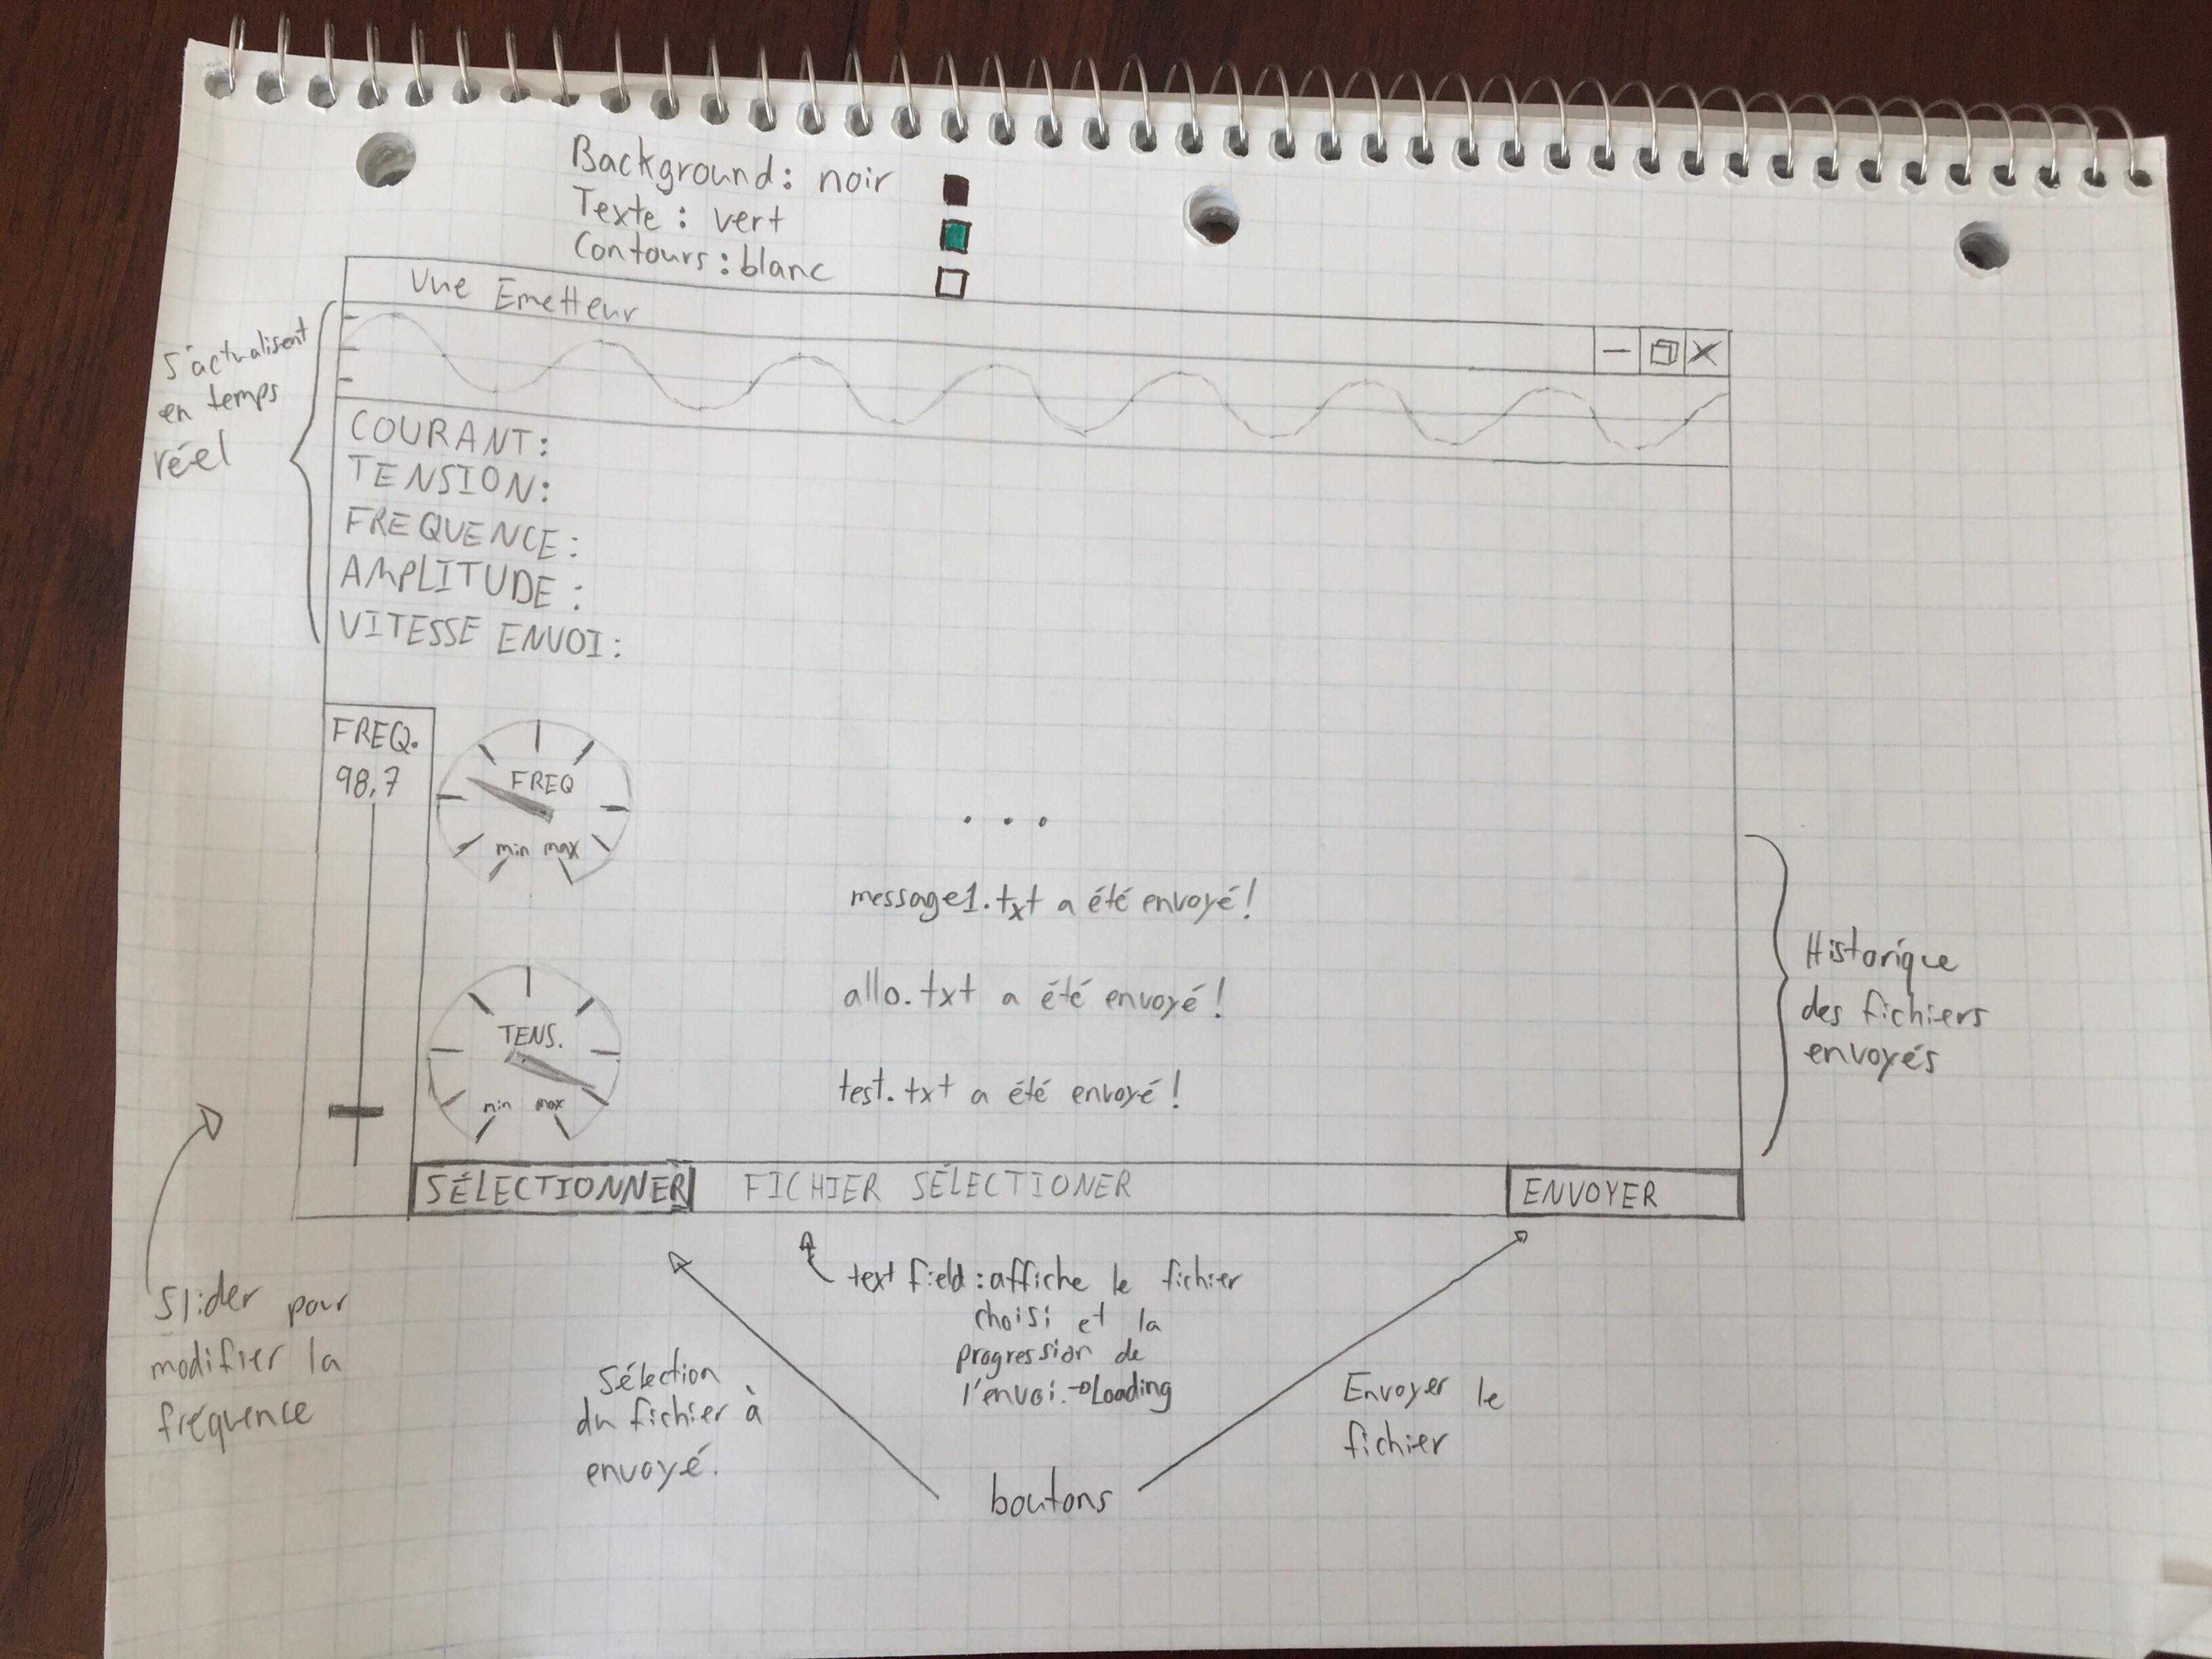
\includegraphics[width=0.8\linewidth]{images/proto/interface_graphique.jpg}
\end{figure}

\newpage

\paragraph{Principaux objets :} 
\begin{itemize}
    \item Visualisation des ondes envoyées
    \item Valeurs pour les différents paramètres 
    \begin{itemize}
        \item Courant dans le circuit
        \item Tension sur le circuit
        \item Fréquence sur laquelle on émet
        \item Amplitude des ondes
        \item Vitesse d'envoi (B/sec ou KB/sec)
    \end{itemize}
    \item La liste des fichiers envoyés
    \item Des boutons pour choisir un fichier et l'envoyer
    \item Un contrôle pour modifier la fréquence
    \item Des visualisations pour la fréquence et la tension relative (pour savoir si on s'approche du maximum permis)
    \item Potentiellement à ajouter serait un indicateur de puissance utilisée par le circuit
\end{itemize}

\begin{figure}[ht!]
    \centering
    \caption{Prototype du physique}
    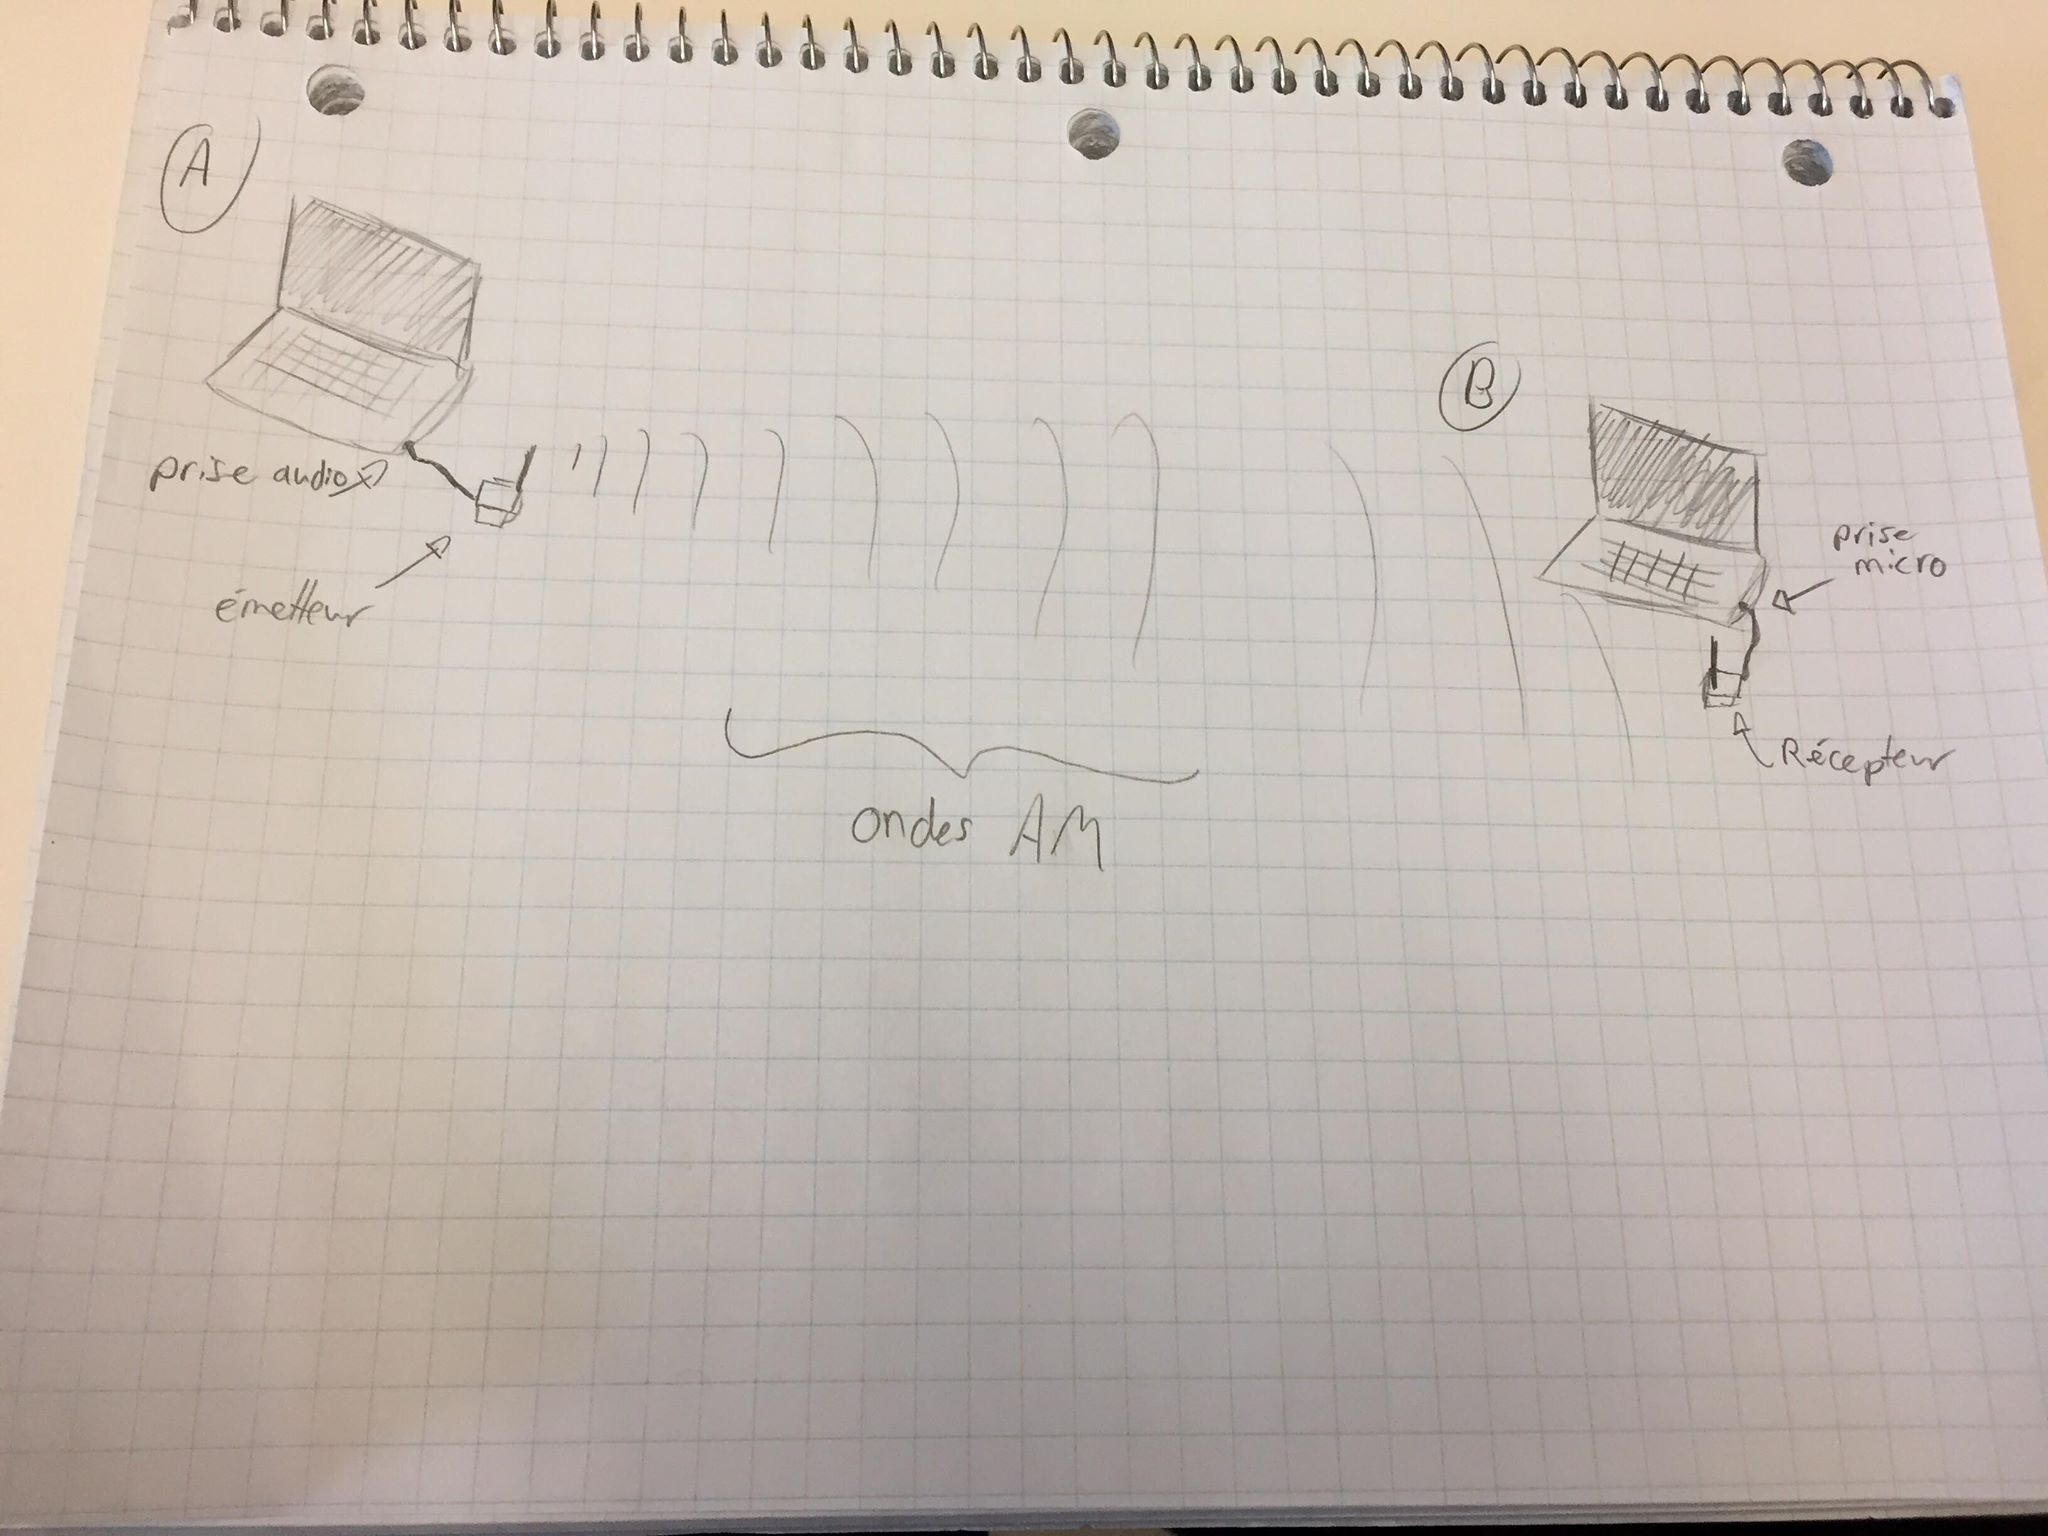
\includegraphics[width=0.4\linewidth]{images/proto/visualisation_transmission.jpg}
\end{figure}